\chapter{Processes}

Processes are both Tasks and ISRs category 2. Trampoline category 2 ISRs are like Basic Tasks except the priority level of the interrupt controller is raised to the priority of the ISR while the later is running.

\section{The States of a Process}

A process has a state used by trampoline to perform various actions on the executable when it executes a service. States include those found at page 17 and 18 of the OSEK/VDX specification \ref{osek:taskstate} and 2 extra states used for internal management. The state is coded using 3 bits as shown in table \ref{processstates}.

\begin{table}[htdp]
\caption{States of a process}
\begin{center}
\rowcolors{1}{white}{light-gray}
\begin{longtablev}{c|c|c|c|l}{}{Decimal value}{bit 2}{bit 1}{bit 0}{Meaning}
\linev{0}{0}{0}{0}{SUSPENDED}
\linev{1}{0}{0}{1}{READY}
\linev{2}{0}{1}{0}{RUNNING}
\linev{3}{0}{1}{1}{WAITING}
\linev{4}{1}{0}{0}{AUTOSTART}
\linev{5}{1}{0}{1}{READY\_AND\_NEW}
\end{longtablev}
\end{center}
\label{processstates}
\end{table}%

Figure \ref{fig:states} shows how a process goes from state to state during the lifetime of an application.

\paragraph{AUTOSTART}

This state is used to indicate what task should be started automatically when StartOS is called. An AUTOSTART task is in this initial state but no task should be in this state when the application code is running.

\paragraph{READY\_AND\_NEW}

This state is used to flag a process that is ready but has its context unitialized. This happens when the process has just been activated. The kernel initializes the context of the process the first time it goes to the RUNNING state.

\begin{figure}[htbp] %  figure placement: here, top, bottom, or page
   \centering
   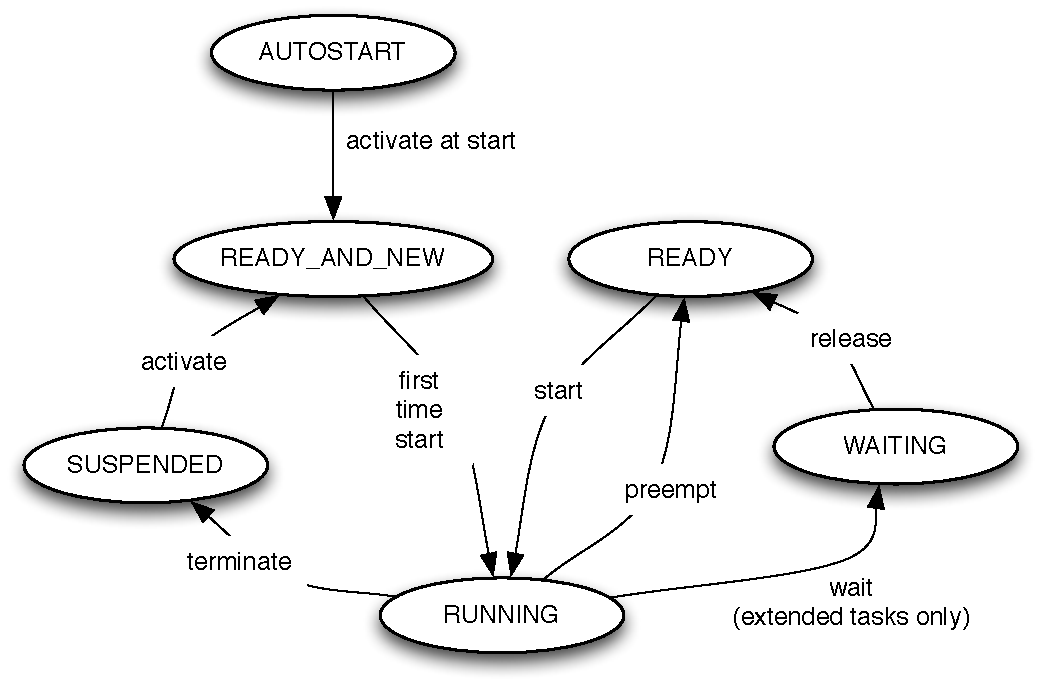
\includegraphics[width=4in]{pictures/states.pdf} 
   \caption{States of a process in Trampoline. AUTOSTART is the initial state of autostart tasks. SUSPENDED is the initial state of both non autostart tasks and ISR category 2.}
   \label{fig:states}
\end{figure} 